\documentclass[tikz,border=8pt]{standalone}
\usepackage[utf8]{inputenc}
\usepackage{xcolor}
\usepackage{amsmath}
\usetikzlibrary{arrows.meta,calc,positioning,fit}
\renewcommand{\familydefault}{\sfdefault}

\definecolor{medBlue}    {HTML}{4A86B8}
\definecolor{branchA}    {HTML}{C97B4A}
\definecolor{branchB}    {HTML}{4A86B8}
\definecolor{branchC}    {HTML}{6FA888}
\definecolor{panelGray}  {HTML}{CFCFCF}

\tikzset{
  font=\sffamily\large,
  arrow/.style={-{Latex[length=3mm,width=2.4mm]},draw=black,line width=1.4pt},
  panel/.style={rounded corners=10pt,draw=panelGray,dashed,line width=1.6pt,fill=white},
  data/.style={rectangle,rounded corners=3pt,draw=black!50,line width=1.1pt,fill=black!6,
    minimum width=4.8cm,minimum height=2.0cm,align=center,inner xsep=8pt,font=\large\itshape},
  modelA/.style={rectangle,rounded corners=3pt,draw=none,fill=branchA,text=white,
    minimum width=4.6cm,minimum height=1.8cm,align=center,inner xsep=8pt,font=\bfseries\large},
  modelB/.style={rectangle,rounded corners=3pt,draw=none,fill=branchB,text=white,
    minimum width=4.6cm,minimum height=1.8cm,align=center,inner xsep=8pt,font=\bfseries\large},
  modelC/.style={rectangle,rounded corners=3pt,draw=none,fill=branchC,text=white,
    minimum width=4.6cm,minimum height=1.8cm,align=center,inner xsep=8pt,font=\bfseries\large},
  scorebox/.style={rectangle,rounded corners=3pt,line width=1.2pt,
    minimum width=3.6cm,minimum height=1.6cm,align=center,inner xsep=6pt,font=\bfseries\large},
  merge/.style={rectangle,rounded corners=3pt,fill=medBlue!18,draw=medBlue,line width=1.3pt,
    minimum width=5.4cm,minimum height=3.0cm,align=center,font=\bfseries\large,text=black},
  title/.style={font=\sffamily\bfseries\huge,align=center},
}

\begin{document}
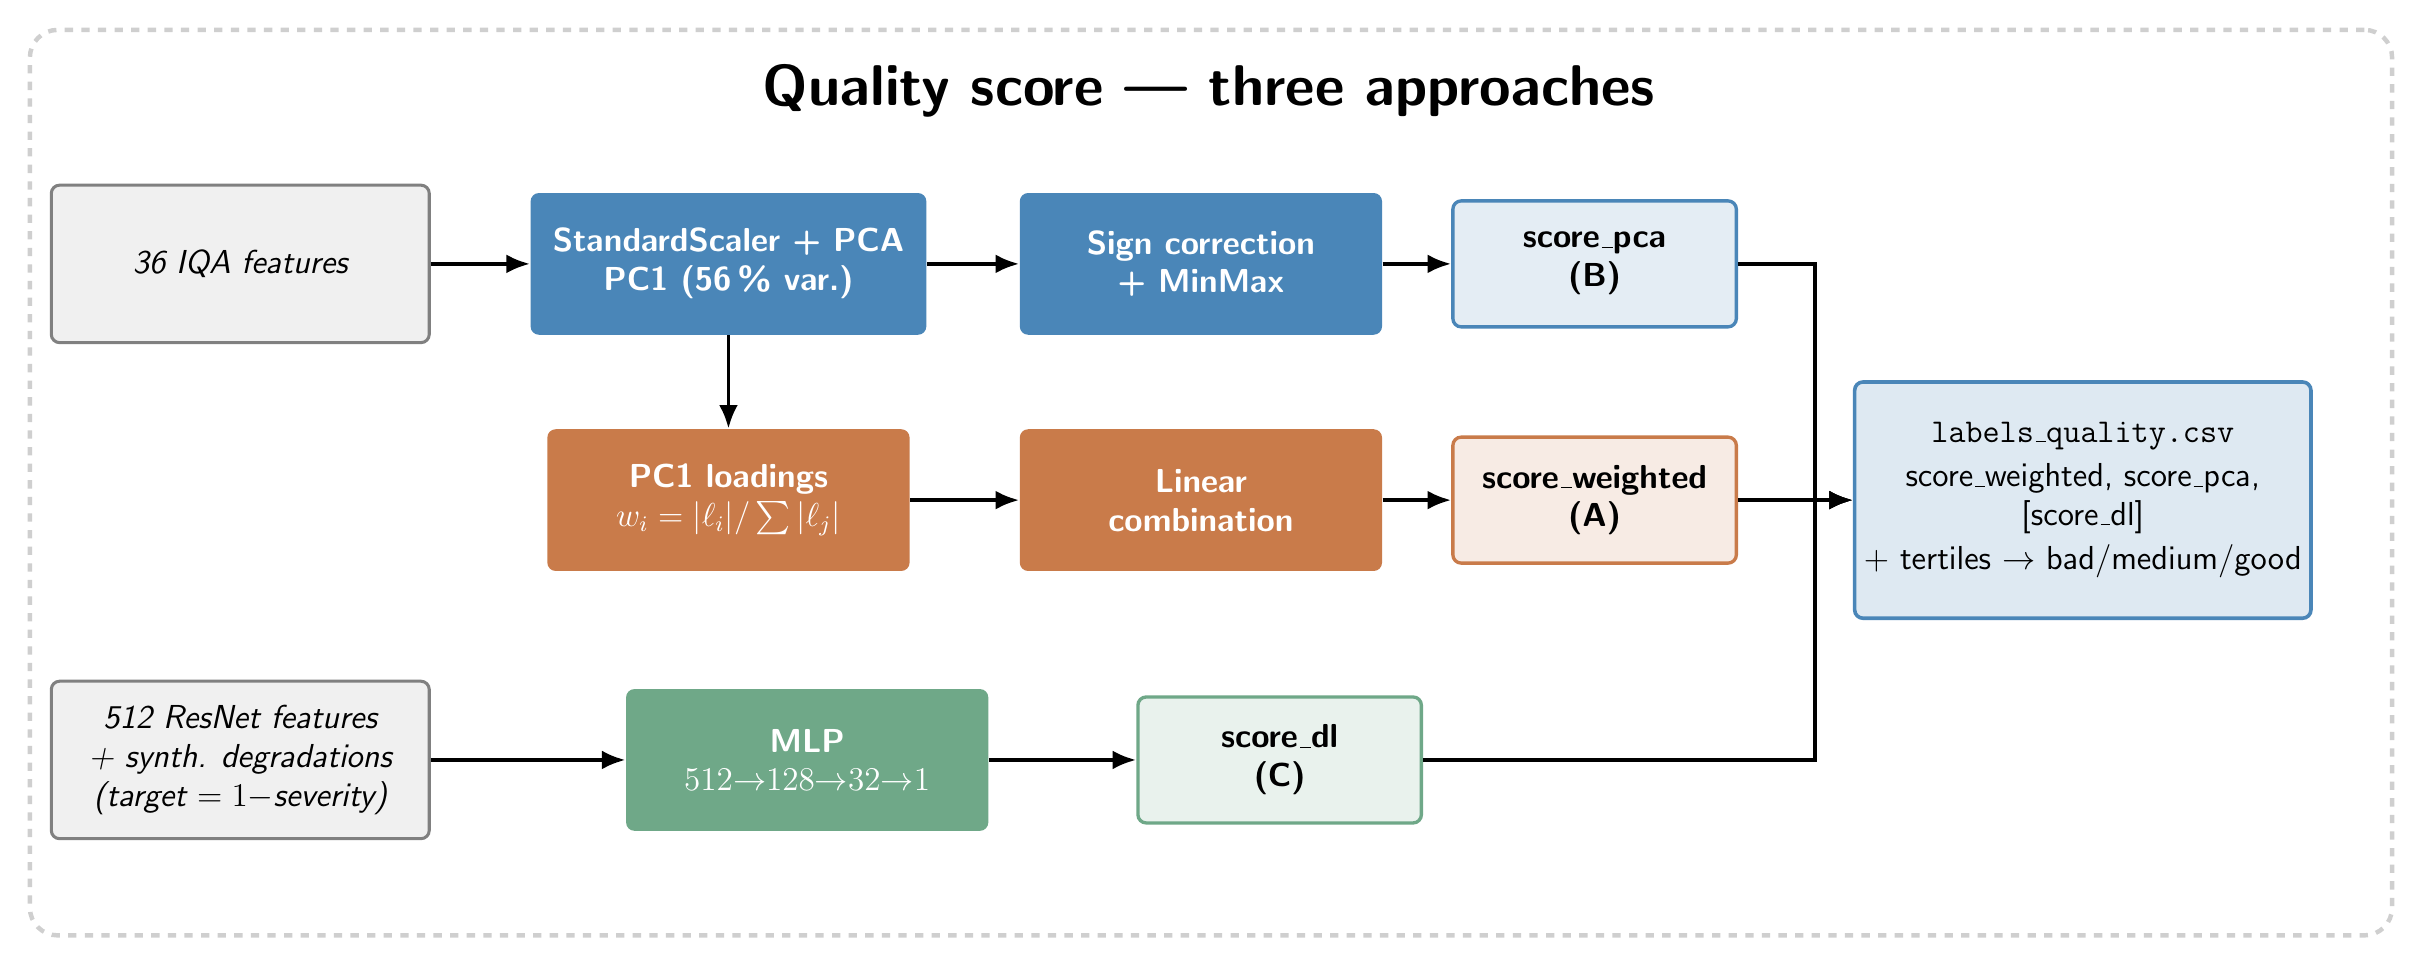
\begin{tikzpicture}[x=1cm,y=1cm]

\node[panel,minimum width=30cm,minimum height=11.5cm,anchor=north west] at (-.3,11.3){};

\node[title] at (14.7,10.5) {Quality score --- three approaches};

\node[data] (feat36) at (2.4,8.3) {36 IQA features};

\node[modelB] (pca) at (8.6,8.3) {StandardScaler + PCA\\PC1 (56\,\% var.)};
\node[modelB] (signB) at (14.6,8.3) {Sign correction\\+ MinMax};
\node[scorebox,draw=branchB,fill=branchB!15] (scoreB) at (19.6,8.3) {score\_pca\\(B)};

\draw[arrow] (feat36.east) -- (pca.west);
\draw[arrow] (pca.east) -- (signB.west);
\draw[arrow] (signB.east) -- (scoreB.west);

\node[modelA] (loadings) at (8.6,5.3) {PC1 loadings\\$w_i=|\ell_i|/\sum|\ell_j|$};
\node[modelA] (combA) at (14.6,5.3) {Linear\\combination};
\node[scorebox,draw=branchA,fill=branchA!15] (scoreA) at (19.6,5.3) {score\_weighted\\(A)};

\draw[arrow] (pca.south) -- (loadings.north);
\draw[arrow] (loadings.east) -- (combA.west);
\draw[arrow] (combA.east) -- (scoreA.west);

\node[data] (feat512) at (2.4,2.0) {512 ResNet features\\+ synth. degradations\\(target $=1{-}$severity)};
\node[modelC] (mlp) at (9.6,2.0) {MLP\\$512{\to}128{\to}32{\to}1$};
\node[scorebox,draw=branchC,fill=branchC!15] (scoreC) at (15.6,2.0) {score\_dl\\(C)};

\draw[arrow] (feat512.east) -- (mlp.west);
\draw[arrow] (mlp.east) -- (scoreC.west);

\node[merge] (merge) at (25.8,5.3)
  {\texttt{labels\_quality.csv}\\[2pt]{\large\mdseries score\_weighted, score\_pca,}\\{\large\mdseries [score\_dl]}\\[2pt]{\large\mdseries + tertiles $\to$ bad/medium/good}};

\draw[arrow] (scoreB.east) -- (22.4,8.3) -- (22.4,5.3) -- (merge.west);
\draw[arrow] (scoreA.east) -- (merge.west);
\draw[arrow] (scoreC.east) -- (22.4,2.0) -- (22.4,5.3) -- (merge.west);

\end{tikzpicture}
\end{document}
